\documentclass[12pt,letter]{article}
\usepackage{../downey_format}

\begin{document}
	
	% set the section number, along with figure and equation numbers
	\setcounter{section}{6}	
	\setcounter{figure}{0}   
	\renewcommand\thefigure{\thesection.\arabic{figure}}
	\setcounter{equation}{0}   
	\renewcommand\theequation{\thesection.\arabic{equation}}

	\section{Experimental Vibrations}
	
Experimental testing requires the practitioner to understand the basics of testing hardware and digital signal processing. An understanding of how to acquire and process vibration data is key to being able to apply one's knowledge of vibrations to real-world systems.


\begin{vibration_case_study}

	\textbf{Challenges in Structural Monitoring}	

	\noindent On August 14, 2018, the Ponte Morandi viaduct in Genoa Italy collapsed, killing 43 and displacing hundreds of people from their homes. The Morandi viaduct was a cable-stayed bridge with uniquely few stays, typically only two per span. The Stays were a hybrid of steel cables overlaid with concrete. The concrete overlay made the direct inspection of the stays impossible. 
	
	While the exact cause may never be known, is suspected that one of the stay cables within the concrete failed due to corrosion and poor maintenance causing a bridge with very little redundancy in its design to fail\protect\footnotemark[1].
	
	In 2017, researchers from the Polytechnic University of Milan instrumented and studied the vibration characteristics of the bridge and noted that the modal frequencies of the stays on pillar 9 (the one that collapsed) were more than 10\% different than other stays on the bridge. While it's always hard to draw conclusions from one test, comparing modal frequencies between two similar structures can be useful for tracking damage. 
 
	\begin{figure}[H]
		\centering
		\includegraphics[width=6in]{../figures/ponte_morandi_bridge}
		\caption{The Ponte Morandi bridge, showing the bridge: a) before the collapse\protect\footnotemark[2], and; b) after collapse\protect\footnotemark[3]. }
	\end{figure}
		
	\footnotetext[1]{Rymsza, Janusz. ``Causes of the Collapse of the Polcevera Viaduct in Genoa, Italy.'' Applied Sciences 11, no. 17 (2021): 8098. https://doi.org/10.3390/app11178098.} 	
	\footnotetext[2]{Davide Papalini, CC BY-SA 3.0 $<$https://creativecommons.org/licenses/by-sa/3.0$>$, via Wikimedia Commons} 
	\footnotetext[3]{Michele Ferraris, CC BY-SA 4.0 $<$https://creativecommons.org/licenses/by-sa/4.0$>$, via Wikimedia Commons} 
\end{vibration_case_study}
		
		
		\begin{figure}[H]
			\centering
			\includegraphics[]{../figures/vibration_testing.png}
			\caption{Key components for performing experimental modal analysis.}
			\label{fig:vibration_testing}
		\end{figure} 
		


The measurement of vibrating systems requires specialized hardware. While a variety of vendors sell vibration measurement systems in a number of form factors, the general hardware requirements remain constant. The basic hardware requirements are: \emph{Exciter} - A system to provide a measurable input to the system, \emph{Transducers} - Sensors used for converting the mechanical movements of the structure to signals, and \emph{data acquisition} - Hardware for digitizing the signal generated by the transducers. Figure~\ref{fig:vibration_testing} shows some of the key systems required for vibration testing and their interactions. 



\subsection{Sensing and Data Acquisition}

The output of a vibrating system is measured through a combination of sensors and data acquisition systems. 

\subsubsection{Accelerometers}

Accelerometers are by far the most common type of sensor used for measuring vibrations. Various types of Accelerometers exist, including Micro-electromechanical systems (MEMS) based systems that are commonly found in cell phones, piezo-resistive-based systems used for high acceleration loading (greater than 10,000 g$_\text{n}$), or piezo-electric sensors commonly deployed in industrial settings. In terms of dedicated vibration testing, piezo-electric sensors are the most common sensor system. 

Piezo-electric sensors use a piezo-electric material to convert small movements into a small electrical charge (measured in Coulomb) in and out of the piezo-electric material. On its own, the signal encoded by this charge is hard to measure and susceptible to electromagnetic noise if run over medium to long wires. Therefore, amplifiers are added to the sensors to assist in transferring this signal back to the data acquisition; thereby creating Integrated Electronics Piezo-Electric (IEPE) sensors. Figure~\ref{fig:accelerometers}(a) shows the cross section of a common IEPE sensor. Through tuning the piezo-electric material and packaging, IEPE sensors can be made to measure a variety of applications (figure~\ref{fig:accelerometers}(b)). Table~\ref{table:accelerometers} reports specifications for five different IEPE sensors that are used to measure a range of applications from the structural motion of buildings to packages subjected to high-shock loading (e.g., missals, plane crashes).

\begin{figure}[H]
    \centering
    \includegraphics[width=6.5in]{../figures/accelerometers}
    \caption{Integrated Electronics Piezo-Electric (IEPE) accelerometers, showing: (a) the cross-section of a typical IEPE) accelerometer with key components annotated, and; (b) selection of IEPE accelerometers for various applications.}
    \label{fig:accelerometers}
\end{figure} 

\begin{table}[H]
\caption{Specifications for various IEPE accelerometers.}
\label{table:accelerometers}
\resizebox{\textwidth}{!}{\begin{tabular}{@{}llllll@{}}
\toprule
\multicolumn{1}{c}{specifications} & \multicolumn{5}{c}{accelerometers} \\ \midrule
model number & PCB 393B31 & PCB  393B04 & PCB 352C67 & PCB 352A21 & PCB 352A92 \\
Sensitivity($\pm$ 10 \%) & 10.0 V/g & 1000 mV/g & 100 mV/g & 10 mV/g & 0.25 mV/g \\
Measurement Range & $\pm$ 0.5 g pk & $\pm$ 5 g pk & $\pm$ 50 g pk & $\pm$ 500 g pk & $\pm$ 20 kg pk \\
Frequency Range($\pm$ 5 \%) & 0.1 to 200 Hz & 0.06 to 450 Hz & 0.5 to 10 kHz & 1.0 to 10 kHz & 1.2 to 10 kHz \\
Resonant Frequency & \textgreater 700 Hz & \textgreater 2.5 kHz & \textgreater 35 kHz & \textgreater 50 kHz & \textgreater 100 kHz \\
Non-Linearity & $\le$1\% & $\le$1\% & $\le$1\% & $\le$1\% &  \\
Transverse Sensitivity & $\le$5\% & $\le$5\% & $\le$5\% & $\le$5 \% &  \\ \bottomrule
\end{tabular}}
\end{table}




\begin{figure}[H]
	\centering
	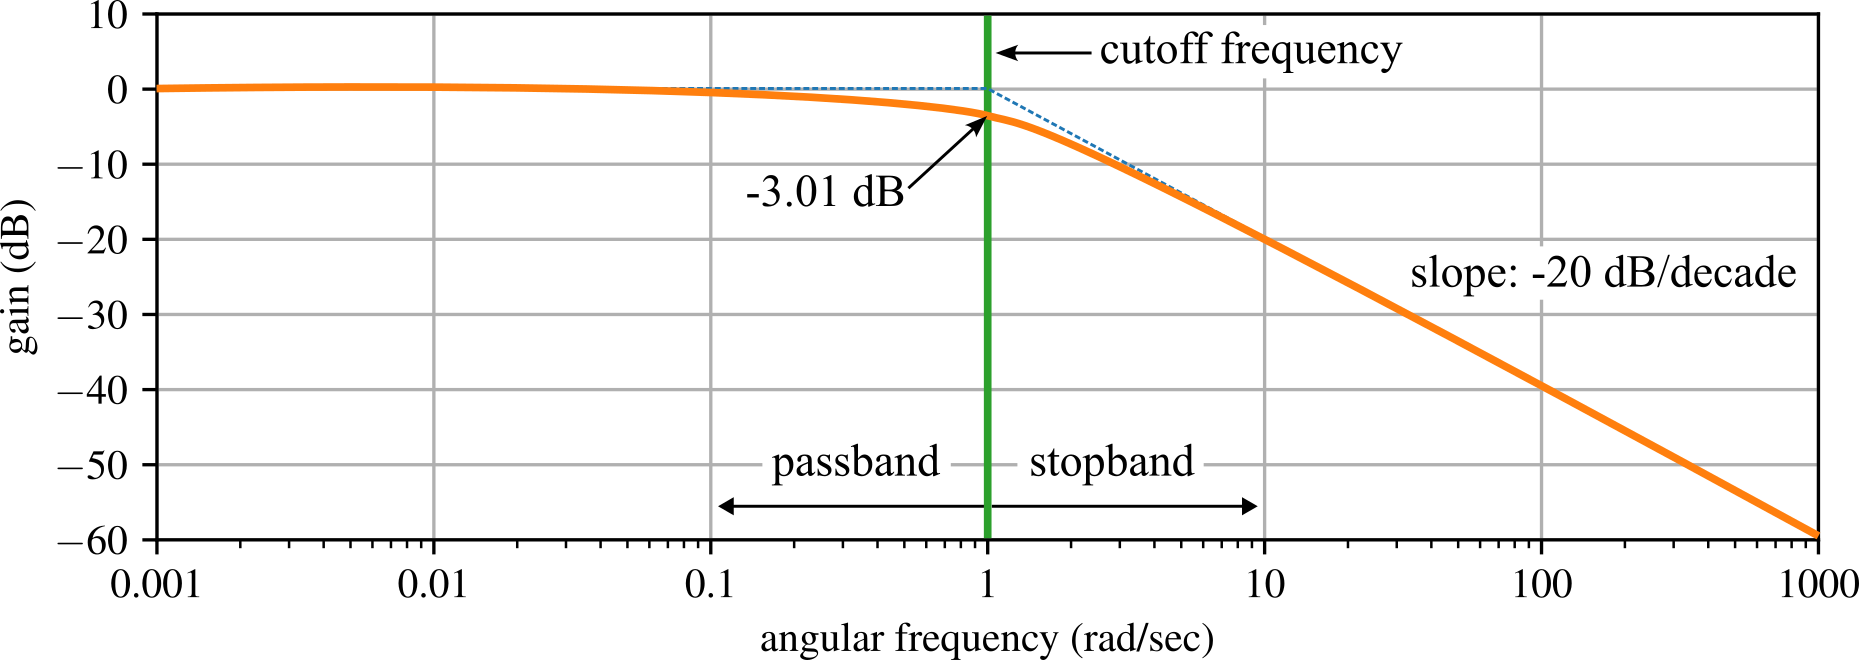
\includegraphics[width=6.198in]{../figures/frequency_rolloff}
	\caption{Graph of a generic frequency roll-off where the cutoff frequency is at -3.01 dB\protect\footnotemark[1].}
	\label{fig:frequency_rolloff}
\end{figure}

\footnotetext[1]{PDerivative work:  KrishnavedalaOriginal:  Omegatron, CC BY-SA 3.0 $<$https://creativecommons.org/licenses/by-sa/3.0$>$, via Wikimedia Commons}



The \emph{frequency range} of a sensor reports the frequency of vibration the sensor is designed to acquire. The upper limit is defined as the cutoff frequency of the sensor which is typically defined as the frequency at which the sensor experiences -3.0~dB (relative unit) of signal power loss. However, at -3.0 dB the power of the measured signal is about half as strong as that of the ideal signal. Figure~\ref{fig:frequency_rolloff} shows a generic frequency roll-off chart. For the practitioner, it is important to note that the signal starts to die off well before the cutoff frequency. Therefore, it is important to be cognizant of a sensor's frequency response when trying to obtain measurements of signals near the upper end of an accelerometer. 





\subsubsection{Data Acquisition}

Acquiring data from sensors was once a challenging task that has been greatly simplified by the development of modern hardware and software systems that are far too numerous to list here. One important item to note here is that IEPE sensors require IEPE data acquisition system, as shown in figure~\ref{fig:IEPE}.  As IEPE sensors generate very small signals, they require amplification before they can be accurately measured. Therefore, an IEPE data acquisition system consists of a front-end amplifier that is specifically designed to amplify these small signals, a signal conditioning circuit that filters and shapes the signals, and an analog-to-digital converter (ADC) that converts the analog signals to digital signals to be analyzed by a computer.

\begin{figure}[H]
    \centering
    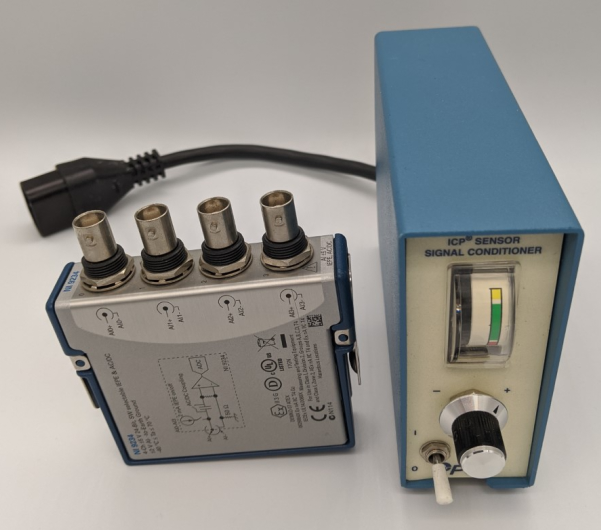
\includegraphics[width=3.0in]{../figures/IEPE.png}
    \caption{Integrated Electronics Piezo-Electric (IEPE) data acquisition systems in various form factors.}
    \label{fig:IEPE}
\end{figure} 






%Measurement Range & 0.5 g pk & \pm 5 g pk & \pm 50 g pk & \pm 100 g pk & \pm 500 g pk & \pm20,000 g pk \\
%Frequency Range(\pm 5 \%) & 0.1 to 200 Hz & 0.06 to 450 Hz & 0.5 to 10,000 Hz & 1 to 5,000 Hz & 1.0 to 10,000 Hz & 1.2 to 10,000 Hz \\

\pagebreak

\subsection{Controlled Force Excitation}

To develop an accurate understanding of vibrating systems, it is important to understand the energy input. Moreover, it is important to test systems under the vibration inputs they may encounter during transportation, operation, or storage as this can help identify potential weaknesses or design flaws in the product.

\subsubsection{Modal Hammers}



\begin{figure}[H]
	\centering
	\includegraphics[width=6.5in]{../figures/modal_hammer}
	\caption{Model hammer, showing: (a) instrumented hammer with interchangeable tips, and; (b) the temporal and frequency response from various tips.}
	\label{fig:modal_hammer}
\end{figure} 


A modal hammer is an instrumented hammer used to impart a measured impact force into the structure. The frequency range of the resulting vibrations is determined by the duration of the impact. A shorter impact duration leads to higher frequencies being excited. To achieve varying frequency bandwidths with the same amount of impact energy, special hammer tips of different stiffnesses can be utilized.  Figure~\ref{fig:modal_hammer} shows a model hammer with interchangeable tips and the responses generated by the tips. In general, there are three factors to be considered when selecting the proper modal hammer.

\underline{Factor 1: Frequency bandwidth.} Softer hammer tips result in longer pulse durations and narrower frequency bandwidths, while harder tips lead to shorter pulse durations and broader frequency bandwidths. However, when using a hard tip, the power spectral density of the excitation may be insufficient to excite vibration modes in the system. In such cases, increasing the impact force by swinging the hammer harder or adding a head extender may be attempted, but there is a risk of overloading the IEPE force transducer. An alternative solution is to switch to a hammer model with a larger measurement range or use a softer tip to concentrate the impact energy at lower frequencies. Moreover, the duration of the pulse may also be affected by the stiffness of the specimen being impacted.

\pagebreak

\underline{Factor 2: Energy of the impact.} The diverse shapes, masses, and material properties (e.g., stiffness or damping) of objects being tested necessitate a range of force pulses with varying parameters to achieve optimal excitation. Compact objects typically have higher resonance frequencies and require less energy to be excited than larger objects. As a result, a short-duration force pulse can be generated using small or medium-sized hammers. In contrast, larger structures require higher-energy impacts, which are typically concentrated in a low-frequency bandwidth. Modal hammers are available in various masses with measurement ranges ranging from 100~N to 20~kN, allowing practitioners to deliver force pulses with different energies without requiring large swings. As large swings make it difficult to control the force and angle of the hammer tip's impact on the structure.

\underline{Factor 3: Tests repeatability.} Hammer impacts performed by the practitioner during testing may vary in terms of impact energy, the frequency bandwidth of excited vibrations, and the angle of impact. Therefore, it is common practice to average multiple results obtained during testing to develop high-quality and consistent data.











\subsubsection{Electrodynamic Shakers}

An electrodynamic shaker can generate a wide range of frequencies and amplitudes that simulate different vibration environments to simulate real-world vibration environments. This is in contrast to a modal hammer that only subjects the measured item to an impulse force. An electrodynamic shaker is shown in figure \ref{fig:vibration_testing}. It consists of a strong electromagnet that generates a magnetic field and a moving coil. When an alternating electrical current is passed through the coil, it generates a magnetic field that interacts with the magnet, causing the instrumented system to vibrate. The vibration produced by the electrodynamic shaker can be controlled by adjusting the frequency, amplitude, and waveform of the electrical signal applied to the coil through an amplifier.



\subsection{Digital Signal Processing}

 An analog signal is a continuous-time signal that can take any value within a certain range, while a digital signal is a discrete-time signal that takes on only a finite number of values at discrete time intervals. Digitization in signal processing is the process of converting an analog signal into a digital form.

\subsubsection{Sampling and Quantization}


The process of digitization involves two main steps: sampling and quantization and is visualized in figure~\ref{fig:signal_digitization} for a sinusoidal and a more complex signal. In the sampling step, the continuous analog signal is measured at regular time intervals, known as the sampling rate; measured in samples-per-second (S/s). The resulting discrete-time signal is a sequence of samples that represent the value of the analog signal at each sampling instant. In the quantization step, each sample is converted from its continuous value to a digital value that can be represented using a finite number of bits. The accuracy of the digitized signal depends on the number of bits used for quantization; the more bits used, the more accurately the signal can be represented.



\begin{figure}[H]
    \centering
    \includegraphics[width=6.5in]{../figures/signal_digitization.png}
    \caption{Digitization of two continuous time-series signals sampled at 5~S/s.}
    \label{fig:signal_digitization}
\end{figure}



	\begin{review}
	\label{sec:Harry_Nyquist}
		
		\textbf{Harry Nyquist}

		\noindent Harry Nyquist (February 7, 1889 - April 4, 1976) was a Swedish physicist and electronic engineer. His parents emigrated to the U.S. in 1907.  He attended the University of North Dakota starting in 1912 where he obtained a B.S. in 1914 and an M.S. in 1915, both in electrical engineering (entry to M.S. was 3 years!). Thereafter, he went to Yale University where he received a Ph.D. in physics in 1917.

		\begin{figure}[H]
			\centering
			\includegraphics[width=2.0in]{../figures/Harry_Nyquist.jpg}
			\caption{Picture of Harry Nyquist from the American Institute of Physics.\protect\footnotemark[1]}
			\label{fig:Harry_Nyquist}
		\end{figure}
		\footnotetext[1]{Fair use, via Wikimedia Commons}
	\end{review}

\subsubsection{Aliasing}





In signal processing, aliasing is an effect that causes different signals to become indistinguishable from each other, as shown in figure~\ref{fig:aliasing}.  In this way, the signals become an alias of one another when sampled. Aliasing accounts for the development of distortion or artifact in a reconstructed signal when compared to the original continuous signal. Aliasing occurs when a continuous-time signal is sampled at a rate that is too low, resulting in a higher-frequency component in the signal being incorrectly represented as a lower-frequency component due to undersampling.

\begin{figure}[H]
    \centering
    \includegraphics[width=6.5in]{../figures/aliasing.png}
    \caption{Aliasing of a 3 Hz signal that is sampled at 5~S/s where the 3 Hz signal folds back on itself to create a 2 Hz signal.}
    \label{fig:aliasing}
\end{figure}

The Nyquist-Shannon sampling theorem is a theorem in the field of signal processing that defines the sample rate that permits a discrete sequence of samples to sample a continuous-time signal of finite bandwidth. It states that a signal must be sampled at a rate at least twice its highest frequency component to be accurately the frequency domain of the signal; this is known as the Nyquist limit. Otherwise, the higher-frequency components of the signal will ``fold'' back into the lower-frequency range, resulting in a distorted representation of the signal. Moreover, the signal must be sampled at twice its highest frequency component with one additional sample to accurately reproduce the temporal domain of the signal. For example, suppose a sine wave with a frequency of 3~Hz is sampled at a rate of 5~S/s; as diagrammed in figure~\ref{fig:aliasing}. According to the Nyquist-Shannon sampling theorem, the signal should be sampled at a rate of at least 6~S/s plus one sample to rebuild the signal in the temporal domain. Because the sampling rate is lower than the Nyquist rate, the higher-frequency component of the signal (3 Hz) will be aliased to a lower frequency (2 Hz), resulting in the distorted representation of the signal shown by the dashed orange line in figure~\ref{fig:aliasing}.

Rebuilding discretely sampled continuous signals requires much more than just sampling at the Nyquist limit of 2$\times$ the desired frequency content of the signal plus one additional data point. This is because the Nyquist limit only applies to rebuilding perfect sinusoidal signals and real-world signals are complex. A good rule of thumb is that a signal must be sampled at least 10 times per cycle to accurately rebuilt the temporal response of the signal.

\subsubsection{Time-Frequency Analysis}


\begin{figure}[H]
    \centering
    \includegraphics[width=6.5in]{../figures/spectrogram.png}
    \caption{Spectrogram of a 0-10 Hz chirp signal.}
    \label{fig:spectrogram}
\end{figure}

The frequency components of a signal can change over time, requiring time-frequency techniques to analyze. Of these, a spectrogram such as that shown in figure~\ref{fig:spectrogram} is a visual representation of the spectrum of frequencies of a signal over time. The spectrogram is created by dividing the signal into short time windows and computing the Fourier transform of each window.  By applying the Fourier transform to each time window of the signal, the spectrogram displays the variation of the frequency content of the signal over time. Spectrograms can be used for a variety of purposes, such as identifying and analyzing patterns in the frequency content of a signal, detecting and visualizing changes in the frequency content over time, and identifying specific frequency components that may be associated with modes of the vibrating system.



% \subsection{Frequency Response Function}


% Add subsections on shock and rotating components






\end{document}














